% PLEASE USE THIS FILE AS A TEMPLATE
% Check file iosart2x.tex for more examples

% add. options: [seceqn,secthm,crcready,onecolumn]
\documentclass[sw]{iosart2x}
\usepackage{hyperref}
%\usepackage{dcolumn}
%\usepackage{endnotes}

%%%%%%%%%%% Put your definitions here


%%%%%%%%%%% End of definitions

\pubyear{0000}
\volume{0}
\firstpage{1}
\lastpage{1}

\begin{document}

\begin{frontmatter}

%\pretitle{}
%Optimization of fragments sizes for route planning over Linked Connections
\title{Linked Connections: the story so far} 
\runningtitle{Article Title}
%\subtitle{}

% For one author:
%\author{\inits{N.}\fnms{Name1} \snm{Surname1}\ead[label=e1]{first@somewhere.com}}
%\address{Department first, \orgname{University or Company name},
%Abbreviate US states, \cny{Country}\printead[presep={\\}]{e1}}
%\runningauthor{N. Surname1}

% Two or more authors:
\author[A]{\inits{D.}\fnms{David} \snm{Chaves-Fraga}\ead[label=e1]{dchaves@fi.upm.es}},
\author[B]{\inits{J.}\fnms{Julian} \snm{Rojas}\ead[label=e2]{julianandres.rojasmelendez@ugent.be}},
\author[B]{\inits{P.}\fnms{Pieter} \snm{Colpaert}\ead[label=e3]{pieter.colpaert@ugent.be}}
and
\author[A]{\inits{O.}\fnms{Oscar} \snm{Corcho}\ead[label=e4]{ocorcho@fi.upm.es}}
\runningauthor{Chaves-Fraga et al.}
\address[A]{Ontology Engineering Group, \orgname{Universidad Polit\'ecnica de Madrid}, \cny{Spain}}
\address[B]{IDLab, Department of Electronics and Information Systems, \orgname{Ghent University-imec}, \cny{Belgium}
\printead[presep={\\}]{e1,e2,e3,e4}}


\begin{abstract}
Deal with the access and the management of static, but also historical and real-time data, is one of the most relevant problems in several domains which want to take advantage of the benefits of Linked Data. The transport domain is one of these domains but, nowadays, their data are exposing in a way that only ad-hoc systems are able to process them. In previous work, the Linked Connections(LC) framework was introduced as a cost-efficient publishing alternative to the \textit{de-facto} GTFS standard and route planning APIs. At the moment that the route planners take into account real-time and historic data, new issues appear, like for example how we should expose the data on the web, how to improve the query performance or how to ensuring data consistence.

In this paper we present the advances made in the LC framework to deal with real-time and historical data in the transport domain providing a light HTTP interface that allows smart clients to create their own route planners. Our main contribution is a LC server, based on the principles of Linked Data Fragments, that is able to specify the size of each fragment, improving the query evaluation performance and providing a robust access to the data. We also implement the memento protocol in the top of LC and create a new metadata model for improving the discoverability of transport datasets. We evaluate and compare our approach with other possibilities that are also able to deal with real time and historic data. We discover that take into account the size of the fragments has a relevant impact in the performance on the route planning algorithms.   

\end{abstract}

\begin{keyword}
\kwd{Linked Connections}
\kwd{Linked Data Fragments}
\kwd{Transport}
\kwd{Historical Data}
\kwd{Real-time Data}
\kwd{Route Planning}
\end{keyword}

\end{frontmatter}

\section{Introduction}\label{introduction} %Oscar and David
As th



\section{Related Work}\label{related_work} %David
On the current state of the Web, huge amount of data are exposed following the principles of Linked Data. We describe the main contributions on this topic, and also the relevance of the ones made in querying data on the web and the current solutions on planning transport routes using semantics.
%about linked data fragments and route planning with semantics
\subsection{Linked Data}
%what is linked data and its benefits
One of the most well-known alternatives to publish data on the Web is Linked Data \cite{bizer2009linked}. Linked Data allows to identify in an unique way resources on the Web using identifiers, or HTTP URIs. It is a method to distribute and scale data over large organizations such as the Web. When looking up this identifier by using the HTTP protocol or using a Web browser, a definition must be returned, including links towards potential other interesting resources, a practice called \textit{dereferencing}. The triple format to be used in combination with URIs is standardized within RDF. The URIs used for these triples already existed in other data sources, and we thus favored using the same identifiers. It is up to a data publisher to make a choice on which data sources can provide the identifiers for a certain type of entities. 

There are multiple benefits of exposing the data on the Web as Linked data: i) the data is linked to related data so the information can be combined across different interfaces, ii) the data is queryable using the query language for RDF, SPARQL \cite{prud2006sparql}, or other approaches like API-Rest interfaces \cite{world2014json} or \cite{lanthaler2013creating} iii) the data is represented following a reference model, so the interoperability between different data sources is at the semantic level.

In transport domain


\subsection{Querying data on the Web}

\subsection{Route planners}



\begin{figure}[h]
	\centering
	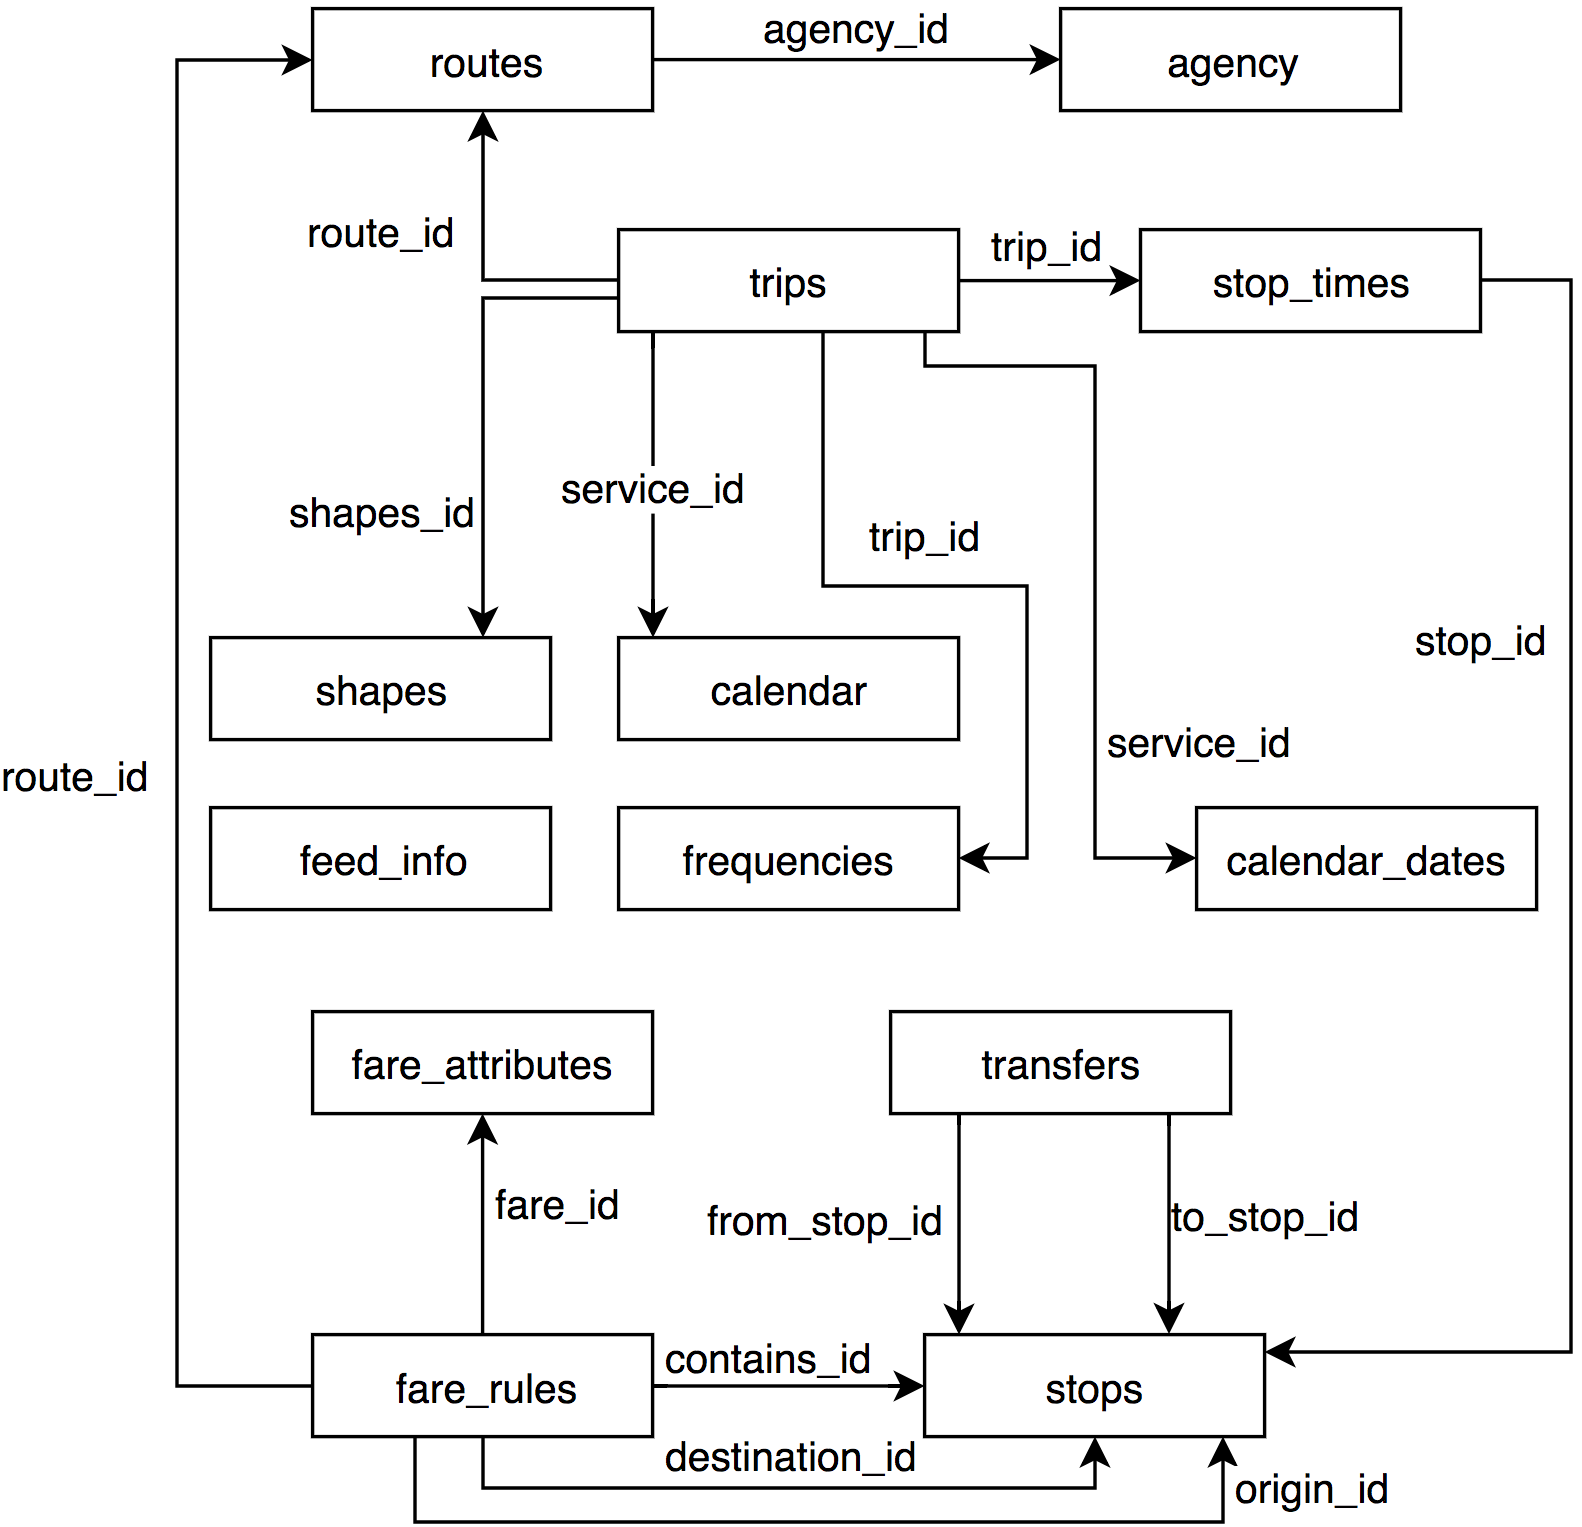
\includegraphics[width=1.0\linewidth]{images/gtfsmodel.png}
	\caption{Underlying GTFS schema}
	\label{fig:gtfs}
\end{figure}

\section{Linked Connections}

\subsection{Linked Connections Server}

\subsection{The Memento Protocol}

\subsection{TransportDCAT-AP}

\section{Evaluation Design}

\section{Results}

\section{Discussion}

\section{Conclusions and Future work}

\begin{acks}

\end{acks}
%%%%%%%%%%%%%%%%%%%%%%%%%%%%%%%%%%%%%%%%%%%%%%%%%%%%%%%%%%%%%
%%                  The Bibliography                       %%
%%                                                         %%
%%  ios1.bst will be used to                               %%
%%  create a .BBL file for submission.                     %%
%%                                                         %%
%%                                                         %%
%%  Note that the displayed Bibliography will not          %%
%%  necessarily be rendered by Latex exactly as specified  %%
%%  in the online Instructions for Authors.                %%
%%                                                         %%
%%%%%%%%%%%%%%%%%%%%%%%%%%%%%%%%%%%%%%%%%%%%%%%%%%%%%%%%%%%%%


\nocite{*} 
% if your bibliography is in bibtex format, use those commands:
\bibliographystyle{ios1}           % Style BST file.
\bibliography{bibliography}        % Bibliography file (usually '*.bib')

% or include bibliography directly:
%\begin{thebibliography}{0}
%\bibitem{r1} F. Author, Information about cited object.
%
%\bibitem{r2} S. Author and T. Author, Information about cited object.
%\end{thebibliography}

\end{document}
